
\newpage
\pagestyle{plain}
\pagenumbering{roman}
%\renewcommand{\thepage}{\Alph{page}}

\section{Plán práce a jeho plnenie}

Plán práce:

\begin{itemize}
	\item DP1:
		\begin{itemize}
			\item analýza problematiky
			\item prvotné experimenty
		\end{itemize}
	\item DP2:
		\begin{itemize}
			\item vybratie vhodného datasetu
			\item experimentovanie s modelmi pozornosti zdola nahor
			\item nájdenie najlepšieho modelu pre ďalšie experimentovanie
		\end{itemize}
	\item DP3:
		\begin{itemize}
			\item experimentovanie so sémantickým kontextom a faktormi pozornosti zhora nadol
			\item výber najlepšieho modelu
			\item testovanie a porovnanie s existujúcimi riešeniami
		\end{itemize}
\end{itemize}

Moje vyjadrenie k plánu práce považujem za irelevantné, rovnako ako samotný plán, nakoľko sa neustále menil a nemalo zmysel ho v jednotlivých semestroch určovať. K riešeniu projektu sme pristúpili agilne, pružne sme reagovali na zmeny a výsledky z jednotlivých experimentov, podľa ktorých sme počas celej práce upravovali jej smerovanie. 
\newpage
\null
\thispagestyle{empty}
\newpage
\section{Obsah priloženého elektronického nosiča}

Štruktúra dát na elektronickom nosiči:

\begin{itemize}
	\item \textbf{datasets} - datasety použité na trénovanie a testovanie, vzorka upraveného pripraveného datasetu pre neurónovú sieť
	\item \textbf{source\_codes\_with\_models} - zdrojové kódy, aj s príslušnými uloženými modelmi
	\item \textbf{source\_codes\_with\_models/autoencoder} - skripty pre trénovanie a predikcie autoenkóderu, uložený jeho natrénovaný model 
	\item \textbf{source\_codes\_with\_models/CNN} - skripty pre trénovanie a predikcie konvolučnej neurónovej siete
	\item \textbf{source\_codes\_with\_models/vgg16\_with\_autoencoder} - skripty pre trénovanie a predikcie autoenkóderu s VGG16 sieťou, uložený natrénovaný najlepší model
	\item \textbf{source\_codes\_with\_models/nn\_utils} - zdrojové kódy pomocných skriptov (napr. pre načítanie dát, výpočet máp fixácií, výpočet metrík atď.)
	\item \textbf{source\_codes\_with\_models/salicon\_api} - aktualizované skripty pre prácu so salicon datasetom
	\item \textbf{document} - pdf verzia odovzdávanej práce
\end{itemize}
\newpage
\null
\thispagestyle{empty}

\newpage
\section{Technická dokumentácia}
\label{technical_doc}

Celé popisované riešenie bolo vyvinuté a otestované na Linux-ových operačných systémoch Ubuntu 18.04.2 LTS a Fedora 28 - na nich vieme  zaručiť správne korektné fungovanie priložených skriptov. Tie sú napísané v jazyku Python vo verzii 3.5, za použitia nasledovných knižníc:

\begin{itemize}
	\item TensorFlow - vo verzii 1.13.1, knižnica pre prácu s neurónovými sieťami 
	\item Keras - vo verzii 2.2.2, vysoko úrovňová knižnica pre prácu s neurónovými sieťami, v našom riešení využíva nižšie úrovňový TensorFlow (za použitia napríklad knižnice Theano skripty nebudú fungovať)
	\item Matplotlib - verzia 3.0.0, knižnica pre 2D vykreslovanie a prácu z obrázkami, použitá pri vizualizáciách predikcií
	\item OpenCV - verzia 3.4.4.19, knižnica pre počítačové videnie a strojové učenie, použitá pre prácu s obrázkami
	\item SciPy\footnote{https://docs.scipy.org/doc/scipy/reference/index.html} - verzia 1.1.0, knižnica pre prácu s dátami
	\item NumPy\footnote{https://www.numpy.org/} - verzia 1.15.2, knižnica pre prácu s dátami
	\item Image Processing SciKit (scikit-image)\footnote{https://scikit-image.org/} - verzia 0.14.1, knižnica pre jednoduché spracovanie obrázkov
\end{itemize}

Verzie knižníc uvádzame z dôvodu kompatibility riešenia, napríklad je možné, že skripty budú fungovať aj na iných verziách knižníc pre prácu s neurónovými sieťami (Keras, TensorFlow), ale v iných verziách nemusia byť schopné načítať uložené modely. 

Čo sa týka hardvérového vybavenia, celé riešenie bolo natrénované na grafickej karte Nvidia GeForce GTX 1080 Ti s veľkosťou 12gb a RAM s veľkosťou 32gb. Trénovanie aj predikcie je možné uskutočnovať aj na CPU, bude to však mať značné dopady na výkon. Trénovanie je možné aj na menšej grafickej karte, je však nutné zmenšiť aj veľkosť dávky (z angl. batch size) pre jedno trénovanie.
\newpage
\null
\thispagestyle{empty}
\newpage
\section{Používateľská príručka}

V zásade každý z modelov uvedených v návrhu má jeden priečinok, v ktorom sú jeho príslušné zdrojové kódy a do ktorého sa ukladajú natrénované modely a predikcie. Každý z nich má 2 základné skripty pre trénovanie a predikovanie, ktoré majú niekoľko konfiguračných možností:

\begin{itemize}
	\item konvolučná neurónová sieť:
		\begin{itemize}
			\item \textbf{train.py} - trénovací skript, ako argumenty berie priečinok s obrázkami, mapami, ich veľkosť, počet epoch, veľkosť dávky a model, kde sa má natrénovaná sieť uložiť. Príklad volania: \textbf{\textit{python3 train.py -{}-images dataset/images-train -{}-maps dataset/maps-train -{}-n 64 -{}-batch 100 -{}-epochs 500 -{}-model model.save}}
			\item \textbf{predict.py} - skript pre predikcie a testovanie, ako argumenty berie vstupné obrázky, natrénovaný model, priečinok kam má uložiť prvých 50 predikcií, priečinok s binárnymi mapami a s originálnymi mapami. Príklad volania: \textbf{\textit{python3 predict.py -{}-images dataset/images-test -{}-maps dataset/maps-test -{}-model model.save -{}-binary\_maps dataset/binary-maps -{}-save\_to predicted\_maps}}
		\end{itemize}
	\item autoenkóder:
		\begin{itemize}
			\item \textbf{autoencoder.py} - trénovací skript, v zásade má ako povinné parametre len priečinok s obrázkami a mapami vizuálnej pozornosti. Nepovinných parametrov je ďaleko viac, od počtu epoch až po počty konvolučných vrstiev a filtrov, všetky ale majú predvolené hodnoty (pre konkrétne čísla treba pozrieť priamo do kódu). Príklad volania: \textbf{\textit{python3 autoencoder.py -{}-maps /home/pbeka/dataset/salicon/maps\_older/train+val/ -{}-images /home/pbeka/dataset/salicon/images/train+val/ -{}-batch 100 -{}-epoch 500 -{}-n 224 -{}-conv\_layers 2}}
			\item \textbf{autoencoder\_predict.py} - skript pre predikcie a testovanie, povinné argumenty sú vstupné obrázky, natrénovaný model, priečinok s binárnymi mapami a s originálnymi mapami. Pre nepovinné parametre treba pozrieť priamo do kódu. Príklad volania: \textbf{\textit{autoencoder\_predict.py -{}-images DUT-OMRON-image-test/  -{}-maps DUT-OMRON-maps-test/ -{}-binary\_maps DUT-OMRON-fixations-test/ -{}-model model.save}}
		\end{itemize}
	\item autoenkóder s VGG16 sieťou:
		\begin{itemize}
			\item \textbf{train\_vgg16\_with\_autoencoder.py} - trénovací skript, povinné parametre sú rovnaké ako pri autoenkóderi. Príklad volania: 
			\textbf{\textit{
			python3 train\_vgg16\_with\_autoencoder.py -{}-images salicon/images/train+val/  -{}-maps salicon/maps\_older/train+val/ -{}-loss binary\_crossentropy -{}-optimizer adadelta -{}-samples 13500 -{}-batch 10}}
			\item \textbf{predict\_vgg16\_with\_autoencoder.py} - skript pre predikcie a testovanie, povinné argumenty sú vstupné obrázky, priečinok s binárnymi mapami a s originálnymi mapami, funkcia chyby a optimizér (podľa nich sa načíta model, pri skripte pre trénovaní je názvom uloženého modelu práve ich kombinácia). Pre nepovinné parametre treba pozrieť priamo do kódu. Príklad volania: 
			\textbf{\textit{python3 predict\_vgg16\_with\_autoencoder.py -{}-images salicon/images/test/ -{}-maps salicon/maps\_older/test/ -{}-binary\_maps salicon/binary\_maps\_2014/ -{}-binary\_format jpg -{}-loss binary\_crossentropy -{}-optimizer adadelta}}
			\item \textbf{train\_another\_dataset.py} - skript pre dotrénovanie modelu na inom datasete. Ako argumenty berie priečinok s obrázkami, mapami a natrénovaný model. Príklad volania: \textbf{\textit{python3 train\_another\_dataset.py -{}-images cat2000/images-train+val  -{}-maps cat2000/maps-train+val -{}-model models\_all\_train/adadelta\_binary\_crossentropy.model}}
		\end{itemize}
	\item upravený backpropagation:
		\begin{itemize}
			\item \textbf{backprop\_change\_predict.py} - skript pre predikcie z VGG16 siete po zmene algoritmu spätného šírenia chyby. Argumentami sú priečninok s obrázkami, mapami vizuálnej pozornosti a mapami fixácií. Príklad volania: \textbf{\textit{python3 backprop\_change\_predict.py -{}-images salicon/images/test/ -{}-maps salicon/maps\_older/test/ -{}-binary\_maps salicon/binary\_maps\_2014/}}
		\end{itemize}
\end{itemize}

\pagenumbering{gobble}
\section{Podrobný diagram architektúry s kombináciou VGG16 a autoenkóderu}
\label{vgg16_autoencoder_architecture_detailed}
\begin{figure}[H]
	\begin{center}
		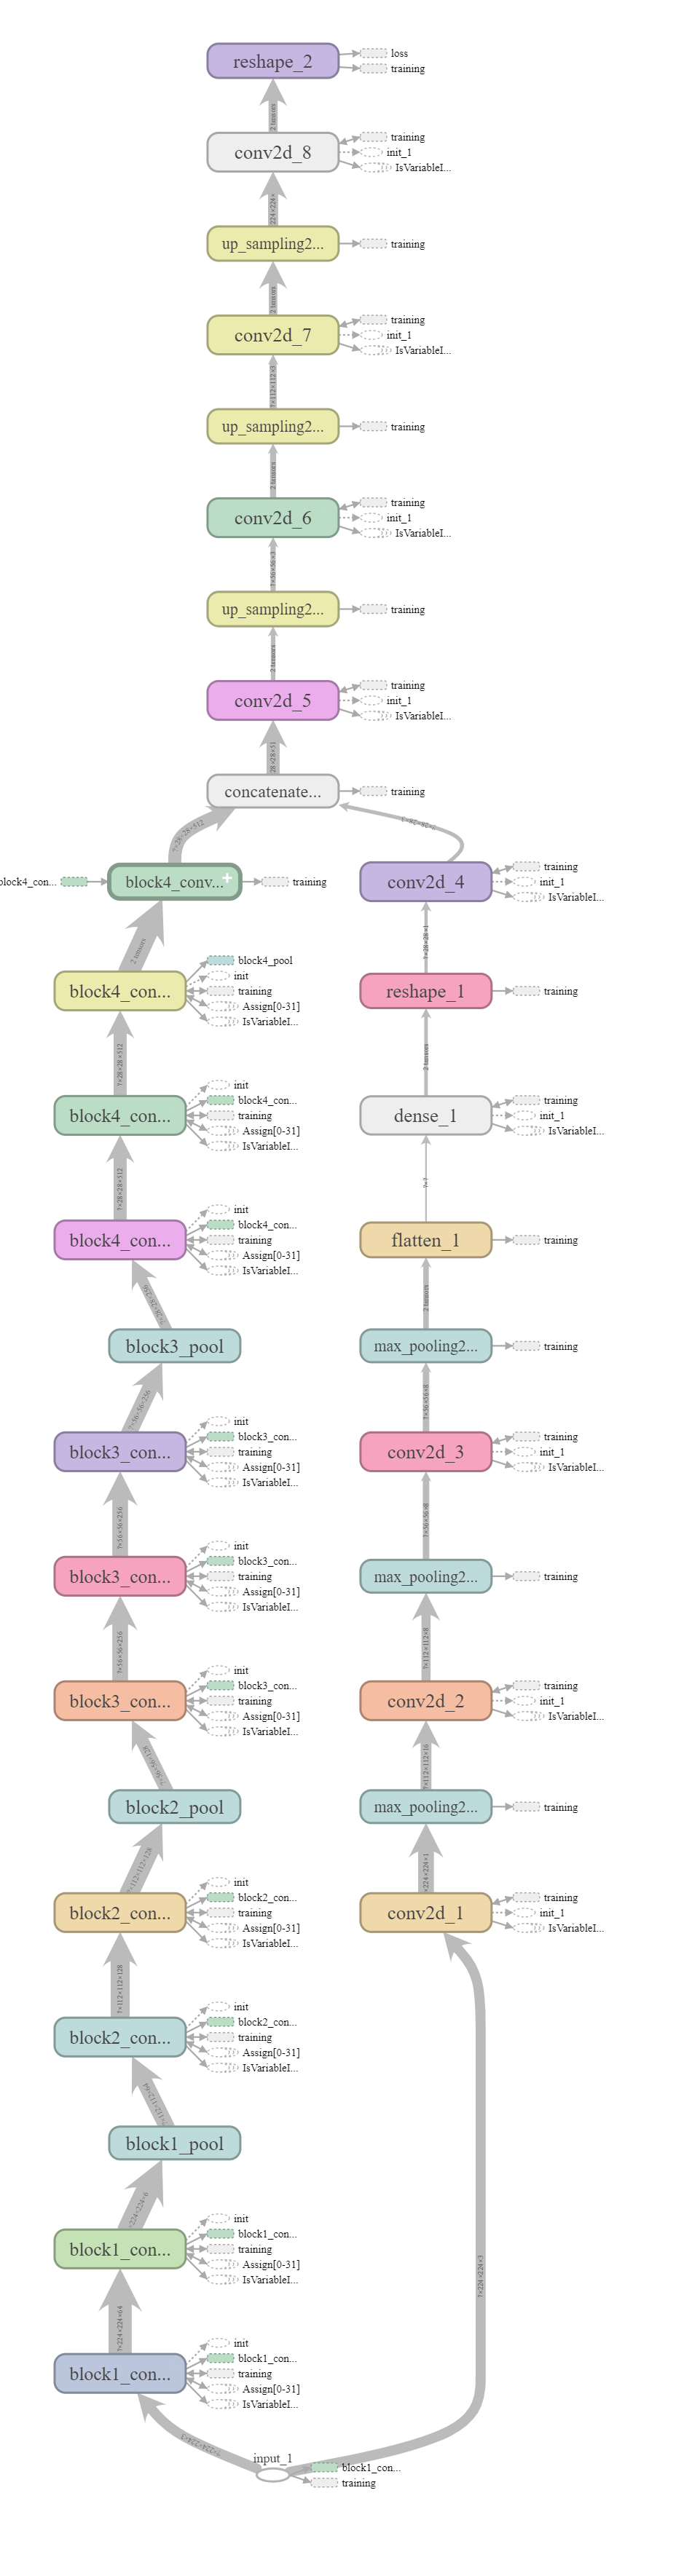
\includegraphics[scale=0.24]{vgg16_with_autoencoder_full.png}
		\caption[Podrobný diagram architektúry VGG16 s autoenkóderom]{Podrobný diagram architektúry VGG16 s autoenkóderom}
	\end{center}
\end{figure}


